%~Mouliné par MaN_auto v.0.23.0 2020-05-14 15:26:36
\documentclass[AHL,Unicode,longabstracts]{cedram}


\DeclareMathOperator{\vol}{Vol}
\DeclareMathOperator{\conv}{conv}

\newcommand*{\dd}{\mathrm{d}}


\newcommand{\wet}[1]{w(#1)}
\newcommand{\eps}{\varepsilon}
\newcommand{\Nbb}{\mathbb{N}}%%\Nbb
\newcommand{\Rbb}{\mathbb{R}}%\Rbb
\newcommand{\Ebb}{\mathbb{E}}%\Ebb
\newcommand{\Hcal}{\mathcal{H}} %%\Hcal


%%désactivés pour l'instant
\newcommand{\pth}[1]{\left(#1 \right)}
\newcommand{\ptb}[1]{\left[#1 \right]}
\newcommand{\blue}[1]{{\color{blue}#1}}


%%\AtBeginDocument{
%\newtheorem{myname}[cdrthm]{My beautiful theorem} }


\newcommand*{\mtfrac}[2]{\frac{#1}{#2}}% si jamais l'auteur veut absolument des tfrac


%%%%%%%%%%%%%%%%%%%%%%%%%%%%%%%%%%%%%%%%%%%%%%%%%%%%

\graphicspath{{./figures/}}

\newcommand*{\mk}{\mkern -1mu}
\newcommand*{\Mk}{\mkern -2mu}
\newcommand*{\mK}{\mkern 1mu}
\newcommand*{\MK}{\mkern 2mu}

\hypersetup{urlcolor=purple, linkcolor=blue, citecolor=red}

\newcommand*{\romanenumi}{\renewcommand*{\theenumi}{\roman{enumi}}}
\newcommand*{\Romanenumi}{\renewcommand*{\theenumi}{\Roman{enumi}}}
\newcommand*{\alphenumi}{\renewcommand*{\theenumi}{\alph{enumi}}}
\newcommand*{\Alphenumi}{\renewcommand*{\theenumi}{\Alph{enumi}}}
%%%%%%%%%%%%%%%%%%%%%%%%%%%%%%%%%%%%%%%%%%%%%%%%%%%%%%%%%

\title[Random polytopes and the wet part]{Random polytopes and the wet part for arbitrary probability distributions}
\alttitle{Polytopes aléatoires et parties immergées de mesures de probabilités arbitraires}

%% pas de \thanks{} avant les \author{}, sinon un auteur fantôme est créé !


% Les noms longs sont trop longs et s'approchent trop du numéro de page.
\author[\initial{I.} \lastname{Bárány}]{\firstname{Imre} \lastname{Bárány}}
\address{Rényi Institute of Mathematics\\
Hungarian Academy of Sciences\\
PO Box 127, 1364 Budapest\\
and Department of Mathematics\\
University College London\\
Gower Street, London WC1E 6BT (UK)}
\email{barany@renyi.hu}

%%[\initial{M.} \lastname{Fradelizi}
\author[\initial{M.} \lastname{Fradelizi}]{\firstname{Matthieu} \lastname{Fradelizi}}
\address{Université Paris-Est, LAMA (UMR 8050)\\
UPEM, UPEC, CNRS\\
77454 Marne-la-Vallée (France)}
\email{matthieu.fradelizi@u-pem.fr}

%%[\initial{X.} \lastname{Goaoc}]
\author[\initial{X.} \lastname{Goaoc}]{\firstname{Xavier} \lastname{Goaoc}}
\address{Université de Lorraine\\
CNRS,Inria, LORIA\\
54000 Nancy (France)}
\email{xavier.goaoc@loria.fr}


%%[\initial{A.} \lastname{Hubard}]
\author[\initial{A.} \lastname{Hubard}]{\firstname{Alfredo} \lastname{Hubard}}
\address{Université Paris-Est, Marne-la-Vallée\\
Laboratoire d'Informatique Gaspard Monge\\
5 Boulevard Descartes\\
77420 Champs-sur-Marne (France)}
\email{alfredo.hubard@u-pem.fr}

%%[\initial{G.} \lastname{Rote}]\mathbb{R}
\author[\initial{G.} \lastname{Rote}]{\firstname{Günter} \lastname{Rote}}
\address{Freie Universität Berlin\\
Institut für Informatik\\
Takustra{\ss}e 9\\
14195 Berlin (Germany)}
\email{rote@inf.fu-berlin.de}

\editor{I. Benjamini}

\subjclass{52B05, 52A22}
\keywords{Random polytope, floating body, $\varepsilon$-nets.}
\thanks{I. B. was supported by the Hungarian National Research, Development and Innovation Office NKFIH Grants K 111827 and K 116769, and by the Bézout Labex (ANR-10-LABX-58). X.~G. was supported by Institut Universitaire de France. The authors are grateful for the hospitality during the ASPAG (ANR-17-CE40-0017) workshop on geometry, probability, and algorithms in Arcachon in April 2018.}

\begin{abstract}
We examine how the measure and the number of vertices of the convex
hull of a random sample of $n$ points from an arbitrary probability measure in $\mathbb{R}^d$ relate to the wet part of that measure. This extends classical results for the uniform distribution from a convex set proved by Bárány and Larman in 1988. The lower bound of Bárány and Larman continues to hold in the general setting, but the upper bound must be relaxed by a factor of $\log n$. We show by an example that this is tight.
\end{abstract}

\begin{altabstract}
Nous examinons comment la mesure et le nombre de sommets de l'enveloppe convexe d'un échantillon aléatoire de $n$ points tirés selon une mesure de probabilité arbitraire sur $\mathbb{R}^d$ sont reliés à la partie immergée de la mesure. Cela étend des résultats classiques pour la mesure uniforme sur un convexe établis par Bárány et Larman en 1988. La minoration de Bárány et Larman est toujours vraie dans ce cadre général mais la majoration doit être affaiblie d'un facteur $\log n$. Nous montrons par un exemple que cette borne est optimale.
\end{altabstract}




\datereceived{2019-02-23}
\dateaccepted{2019-11-08}



\begin{document}

\maketitle


\section{Introduction and Main Results}

Let $K$ be a convex body (convex compact set with non-empty interior) in~$\Rbb^d$, and let $X_n=\{x_1,\ldots,x_n\}$ be a random sample of $n$ uniform independent points from $K$. The set $P_n=\conv X_n$ is a \emph{random polytope} in $K$. For $t\in [0,1)$ we define the \emph{wet part} $K_t$ of $K$:
\[
K_t=\{\,x \in K: \text{there is a halfspace }h \text{ with } x \in h \text{ and }\vol(K\cap h) \le t\vol K\,\}
\]
The name ``wet part'' comes from the mental picture when $K$ is in $\Rbb^3$ and contains water of volume $t\vol K$. Bárány and Larman~\cite{BarLar} proved that the measure of the wet part captures how well $P_n$ approximates $K$ in the following sense:

\begin{theo}[{\cite[Theorem~1]{BarLar}}] \label{th:BL}
There are constants $c$ and $N_0$ depending only on $d$ such that for every convex body $K$ in $\Rbb^d$ and for every $n>N_0$
\[
\frac 14 \vol K_{1/n} \le \Ebb[\vol(K\setminus P_n)] \le \vol K_{c/n}.
\]
\end{theo}

By Efron's formula (see~\eqref{eq:Efron} below), this directly translates into bounds for the expected number of vertices of~$P_n$, see Section~\ref{f-vectors}.

\subsection{Results for general measures.}

The notions of random polytope and wet part extend to a general probability measure $\mu$ defined on the Borel sets of $\Rbb^d$. The definition of a $\mu$-random polytope $P_n^{\mu}$ is clear: $X_n$ is a sample of $n$ random independent points chosen according to $\mu$, and $P_n^{\mu}=\conv X_n$. The wet part $W_t^{\mu}$ is defined as
\[
W_t^{\mu}=\{\,x \in \Rbb^d: \text{there is a halfspace }h \text{ with } x \in h \text{ and }\mu (h) \le t\,\}.
\]
The $\mu$-measure of the wet part is denoted by $w^{\mu}(t):=\mu(W_t^{\mu})$. Here is an extension of Theorem~\ref{th:BL} to general measures:

\begin{theo}\label{th:BLgen}
For any probability measure $\mu$ in $\Rbb^d$ and $n \ge 2$,
\[
\frac 14 w^{\mu}\left(\mtfrac1n\right) \le \Ebb[1-\mu(P_n^\mu)] \le w^{\mu}\left({(d+2)\mtfrac{\ln n}n}\right) + \mtfrac{\varepsilon_d(n)}{n},
\]
where $\varepsilon_d(n)\to 0$ as $n\to+\infty$ and is independent of $\mu$.
\end{theo}

%%\noindent 
A similar upper bound, albeit with worse constants, follows from a result of Vu~\cite[Lemma~4.2]{VanVu}, which states that $P_n^\mu$ contains $\Rbb^d \setminus W_{c\ln n/n}^{\mu}$ with high-probability. Since a containment with high probability is usually stronger than an upper bound in expectation, one may have hoped that the $\log n/n$ in the upper bound of Theorem~\ref{th:BLgen} can be reduced. Our main result shows that this is not possible, not even in the plane:

\begin{theo}\label{th:example}
There exists a probability measure $\nu$ on $\Rbb^2$ such that
\[
\Ebb[1-\mu(P_n^\nu)] > \frac 1{2} \cdot w^\nu(\log_2 n/ n)
\]
for infinitely many $n$.
\end{theo}


The measure that we construct actually has compact support and can be embedded into $\Rbb^d$ for any $d \ge 2$. It will be apparent from the proof that the same construction has the stronger property that for \emph{every} constant $C>0$, the inequality $\Ebb[1-\mu(P_n^\nu)] > \frac 1{2} \cdot w^\nu({C \log_2 n/ n})$ holds for infinitely many values~$n$.


\subsection{Consequences for \texorpdfstring{$\mathbf{f}$}{f}-vectors}\label{f-vectors}

Let $f_0(P_n^\mu)$ denote the number of vertices of $P_n^\mu$. For \emph{non-atomic} measures (measures where no single point has positive probability), Efron's formula~\cite{Ef} relates $E\ptb{f_0(P_n^\mu)}$ and $\Ebb\ptb{\mu(P_n^\mu)}$:
\begin{align}\label{eq:Efron0}
\Ebb [f_0(P_n^\mu)] & = \sum_{i=1}^n \Pr\ptb{x_i \notin \conv(X_n \setminus \{x_i\})}\\
& = n\cdot\int_x \Pr\ptb{x \notin P_{n-1}^\mu}\dd\mu(x) =n(1-\Ebb [\mu(P_{n-1}^\mu)]). \label{eq:Efron}
\end{align}
For \emph{any} measure, this still holds as an inequality:
\begin{equation}\label{eq:Efron2}
\Ebb [f_0(P_n^\mu)] \ge \sum_{i=1}^n \Pr\ptb{x_i \notin \conv(X_n \setminus \{x_i\})} =n(1-\Ebb [\mu(P_{n-1}^\mu)]).
\end{equation}
The measure that is constructed in Theorem~\ref{th:example} is non-atomic. As a consequence, Theorems~\ref{th:BLgen} and~\ref{th:example} give the following bounds for the number of vertices:

\begin{theo}\label{th:fvector}\ \\*[-1.3em]
\begin{enumerate}\romanenumi
\item \label{list.1.4.1} For any non-atomic probability measure $\mu$ in $\Rbb^d$,
\[
\frac 1e n w^{\mu}\left(\mtfrac1n\right) \le \Ebb\ptb{f_0(P_n^\mu)} \le n w^{\mu}\left({(d+2)\mtfrac{\ln n}n}\right) + \varepsilon_d(n),
\]
where $\varepsilon_d(n)\to 0$ as $n\to+\infty$ and is independent of $\mu$.

\item \label{list.1.4.2} There exists a non-atomic probability measure $\nu$ on $\Rbb^2$ such that
\[
\Ebb\ptb{f_0(P_n^\nu)} > \frac 1{2} n \cdot w^\nu(\log_2 n/ n)
\]
for infinitely many $n$.
\end{enumerate}
\end{theo}

%%\noindent
Theorem~\ref{th:fvector} follows from Theorems~\ref{th:BLgen} and~\ref{th:example} except that Efron's Formula~\eqref{eq:Efron} induces a shift in indices, as it relates $f_0(P_n^\mu)$ to $\mu(P_{n-1}^\mu)$. This shift affects only the constant in the lower bound of Theorem~\ref{th:fvector}$\MK$\eqref{list.1.4.1}, which goes from $\frac14$ to $\frac1e$, see Section~\ref{p:lowerbound}.

The upper bound of Theorem~\ref{th:fvector}$\MK$\eqref{list.1.4.1} fails for general distributions. For instance, if $\mu$ is a discrete distribution on a finite set, then $w^\mu(t)=0$ for any $t$ smaller than the mass of any single point and the upper bound cannot hold uniformly as $n \to \infty$. Of course, in that case Inequality~\eqref{eq:Efron2} is strict.

%%\bigskip

For convex bodies, the number $f_i(P_n)$ of $i$-dimensional faces of $P_n$ can also be controlled via the measure of the wet part since Bárány~\cite{Bar} proved that $\Ebb[f_i(P_n)]= \Theta(n \vol K_{1/n})$ for every $0 \le i \le d-1$. No similar generalization is possible for Theorem~\ref{th:BLgen}. Indeed, consider a measure $\mu$ in $\Rbb^4$ supported on two circles, one on the $(x_1,x_2)$-plane, the other in the $(x_3,x_4)$-plane, and uniform on each circle; $P_n^\mu$ has $\Omega(n^2)$ edges almost surely.


%%\bigskip

Before we get to the proofs of Theorems~\ref{th:BLgen} (Section~\ref{s:epsnet}) and~\ref{th:example} (Section~\ref{sec:example}), we discuss in Section~\ref{s:regularity} a key difference between the wet parts of convex bodies and of general measures.


\section{Wet part: convex sets versus general measures}\label{s:regularity}

A key ingredient in the proof of the upper bound of Theorem~\ref{th:BL} in~\cite{BarLar} is that for a convex body $K$ in $\Rbb^d$, the measure of the wet part $K_t$ cannot change too abruptly as a function of $t$: If $c\ge 1$, then
\begin{equation}\label{eq:wet}
\vol K_t \le \vol K_{ct} \le c' \vol K_t
\end{equation}
where $c'$ is a constant that depends only on $c$ and $d$~\cite[Theorem~7]{BarLar}. In particular, a multiplicative factor can be taken out of the volume parameter of the wet part and the upper bound in Theorem~\ref{th:BL} can be equivalently expressed as
\begin{equation}\label{eq:alternative}
\Ebb[\vol(K\setminus P_n)] \le c' \vol K_{1/n}.
\end{equation}
(This is actually the way how the upper bound of Theorem~\ref{th:BL} is formulated in~\cite[Theorem~1]{BarLar}.) This alternative formulation shows immediately that the lower bound of Theorem~\ref{th:BL} (and hence also of Theorem~\ref{th:BLgen}) cannot be improved by more than a constant.


\subsection{Two circles and a sharp drop}

The right inequality in~\eqref{eq:wet} does not extend to general measures. An easy counterexample to the corresponding bound
\begin{equation}\label{eq:wet-general}
w^\mu(ct) \le c' w^\mu (t)
\end{equation}
is the following ``drop construction''. It is a probability measure~$\mu$ in the plane supported on two concentric circles, uniform on each of them, and with measure $p$ on the outer circle. Let~$\tau$ denote the measure of a halfplane externally tangent to the inner circle; remark that $\tau<p/2$. As $t$ is decreased, the measure $w^\mu(t)$ of the wet part drops at $t=\tau$:
\begin{equation}\label{eq:one-drop}
w^\mu(t) =
\begin{cases}
p, & \text{if } t < \tau,\\
1, & \text{if } t \ge \tau.
\end{cases}
\end{equation}
We can make this drop arbitrarily sharp by choosing a small $p$. In particular, for any given $c'$, setting $p < \frac1{c'}$ makes it impossible to fulfill~\eqref{eq:wet-general} when $t$ is chosen in the range $t<\tau<ct$.

\begin{figure}
\centering 
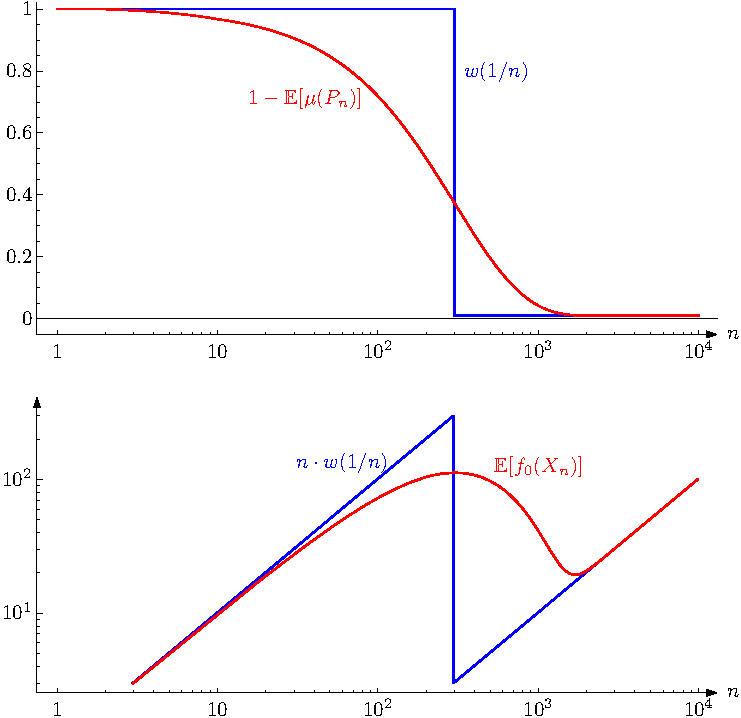
\includegraphics[scale=1]{plotfig3.pdf} 

\caption{The quantities involved in Theorems~\ref{th:BL}--\ref{th:fvector} for the drop construction with $p=1/100$, when the outer circle has twice the radius of the inner circle. Top: $\Ebb[1-\mu(P_n^\mu)]$ and $w(1/n)$, the $x$-axis being a logarithmic scale. Bottom: $\Ebb[f_0(P_n^\mu)]$ and $n\cdot w(1/n)$ on a doubly-logarithmic scale.}\label{fig:example}
\end{figure}

This example also challenges Inequality~\eqref{eq:alternative}. As shown in Figure~\ref{fig:example} (top), the function $w^\mu(1/n)$ has a sharp drop, while $\Ebb\ptb{1-\mu(P_n^\mu)}$ shifts from the higher to the lower branch of the step in a gradual way. For this construction, the straightforward extension of Theorem~\ref{th:BL} would imply that $\Ebb[1-\mu(P_n^\mu)]$ remains within a constant multiplicative factor of $ w^\mu(1/n)$. Thus, $\Ebb[1-\mu(P_n^\mu)]$ would have to follow the steep drop.



\subsection{A drop for the number of vertices.}

The fact that $\Ebb[1-\mu(P_n^\mu)]$ {cannot} drop too sharply is more easily seen by examining $\Ebb\ptb{f_0(P_n^\mu)}$. Since the measure defined in Equation~\eqref{eq:one-drop} is non-atomic, Efron's Formula~\eqref{eq:Efron} applies, so let us compare $\Ebb\ptb{f_0(P_n^\mu)}$ and $n\cdot w^\mu(1/n)$. As illustrated in Figure~\ref{fig:example} (bottom), $n\cdot w^\mu(1/n)$ has a sawtooth shape with a sharp drop from 300 to~3 at $n=300$, and $\Ebb[f_0(P_n)]$ does actually shift from the higher to the lower branch of the sawtooth, in a gradual way.

The fact that $\Ebb[f_0(P_n^\mu)]$ can \emph{decrease} is perhaps surprising at first sight, but this phenomenon is easy to explain: We pick random points one by one. As long as all points lie on the inner circle, $f_0(P_n^\mu)=n$. The first point to fall on the outer circle swallows a constant fraction of the points into the interior of $P_n^\mu$, while adding only a single new point on the convex hull, causing a big drop. This happens around $n\approx 1/p$.


Again, the straightforward extension of Theorem~\ref{th:BL} would imply that $\Ebb[f_0(P_n)]$ follows the steep drop. Yet, on average, a single additional point can reduce $f_0(P_n)$ by {a factor} of at most~$1/2$. Hence, the drop of $\Ebb[f_0(P_n)]$ cannot be so abrupt as the drop of $n\cdot w^\mu(1/n)$, for $p$ small enough.



\subsection{A sequence of drops}

We prove Theorem~\ref{th:example} in Section~\ref{sec:example} by an explicit construction that sets up a sequence of such drops. The function $n\cdot w^\mu(1/n)$ reaches larger and larger peaks as $n$ increases, while dropping down more and more steeply between those peaks. Our proof of Theorem~\ref{th:example} will not actually refer to any drop or oscillating behavior. We will simply identify a sequence of values $n=n_1, n_2, \ldots$ for which $\Ebb[1-\mu(P_{n}^\mu)]$ is larger than $\frac12 w^\mu(\log_2 n/n)$.


\subsection{Open questions}

It is an outstanding open problem whether a drop as exhibited by our two-circle construction can occur for the uniform selection from a \emph{convex} body: Can the expectation of the number of vertices of a random polytope decrease in such a setting? This is impossible in the plane~\cite{DGG} or for the three dimensional ball~\cite{Beermann}, but open in general. See~\cite{BR} and the discussion therein; see also~\cite{KTZ} for the same problem for some particular rotationally invariant measures.

Perhaps Theorem~\ref{th:BL} remains valid for some restricted class of measures~$\mu$, for instance, logconcave measures. One approach to circumvent the ``impossibility result'' of Theorem~\ref{th:example} would be to first extend~\eqref{eq:wet} and establish that for $c>1$ there is $c'$ such that for all $t>0$
\[
w^{\mu}(t) \le w^{\mu}(ct) \le c' \cdot w^{\mu}(t).
\]
The second step would derive from this property the extension of Theorem~\ref{th:BL}. We don't know if any of these two steps is valid.

We can weaken the claim of Theorem~\ref{th:BL} in a different way, while maintaining it for all measures. For example, it is plausible that the upper bound in the theorem holds for a subset of numbers $n \in \Nbb$ of positive density. On the other hand we do not know if there is a measure for which the bound of Theorem~\ref{th:BL} is valid only for a finite number of natural numbers.


\section{Proof of Theorem~\ref{th:BLgen}}\label{sec:proofBLgen}

Let $\mu$ be a probability measure in $\Rbb^d$. For better readability we drop all superscripts~$\mu$.


\subsection{Lower bound}\label{p:lowerbound}
\begin{proof}
The proof of the lower bound is similar to the one in the convex-body case. For every fixed point $x\in W_t$, by definition, there exists a half-space $h$ with $x\in h$ and $\mu(h)\le t$. If $h\cap P_{n}$ is empty, then $x$ is not in $P_{n}$, and therefore, for $x\in W_t$,
\begin{equation}\label{A.}
\Pr[x\notin P_{n}] \ge
\Pr[h\cap P_{n}=\emptyset] = (1-\mu(h))^{n}\ge (1-t)^{n}.
\end{equation}
Then, for any $t$,
\[
\begin{aligned}
1-\Ebb [\mu(P_{n})] & = \int_{x\in \Rbb^d} \Pr[x \notin P_{n}]\dd\mu(x) \\
& \ge \int_{x\in W_t} \Pr[x \notin P_{n}]\dd\mu(x)\\
& \ge \int_{x\in W_t}(1-t)^{n} \dd\mu(x) = (1-t)^{n} w(t).
\end{aligned}
\]
We choose $t=1/n$. Since the sequence $(1-\frac1n)^{n}$ is increasing, for $n \ge 2$ we have $1-\Ebb [\mu(P_{n})] \ge \frac14 w\left(\mtfrac1n\right)$.
\end{proof}

%%\bigskip

To obtain the analogous lower bound from Theorem~\ref{th:fvector}$\MK$\eqref{list.1.4.1}, we write
\[
\Ebb\ptb{f_0(P_n)} = n\Ebb\ptb{1-\mu(P_{n-1})} \ge n(1-t)^{n-1} w(t).
\]
Again, choosing $t=1/n$ yields the claimed lower bound
\[
\Ebb\ptb{f_0(P_n)} \ge n\pth{1-\frac1n}^{n-1} w\left(\mtfrac1n\right)\ge {\frac1e}nw\left(\mtfrac1n\right),
\]
since the sequence $(1-\frac1n)^{n-1}$ is now decreasing to ${\frac1e}$.



\subsection{Floating bodies and \texorpdfstring{$\eps$}{eps}-nets}\label{s:epsnet}

Before we turn our attention to the upper bound, we will point out a connection to $\eps$-nets. Consider a probability space $(U,\mu)$ and a family $\Hcal$ of measurable subsets of $U$. An \emph{$\eps$-net} for $(U, \mu, \Hcal)$ is a set $S\subseteq U$ that intersects every $h\in \Hcal$ with $\mu(h)\ge \eps$~\cite[Section~10.2]{Mat}. In the special case where $U=(\Rbb^d,\mu)$ and $\Hcal$ consists of all half-spaces, if a set $S$ is an $\eps$-net, then the convex hull $P$ of $S$ contains $\Rbb^d\setminus W_\eps$. Indeed, assume that there exists a point $x$ in $\Rbb^d\setminus W_\eps$ and not in $P$. Consider a closed halfspace $h$ that contains $x$ and is disjoint from $P$. Since $x \notin W_\eps$ we must have $\mu(h) > \eps$ and $S$ cannot be an $\eps$-net.

We call the region $\Rbb^d\setminus W_\eps$ the \emph{floating body} of the measure $\mu$ with parameter $\eps$, by analogy to the case of convex bodies. The relation between floating bodies and $\eps$-nets was first observed by Van Vu, who used the $\eps$-net Theorem to prove that $P_n^{\mu}$ contains $\Rbb^d \setminus W_{c\log n/n}$ with high probability~\cite[Lemma~4.2]{VanVu} (a fact previously established by Bárány and Dalla~\cite{BD} when $\mu$ is the normalized Lebesgue measure on a convex body). This implies that, with high probability, $1-\mu(P_n)\le w(c\log n/n)$. The analysis we give in Section~\ref{sec:upperbound} refines Vu's analysis to sharpen the constant. Note that Theorem~\ref{th:example} shows that Vu's result is already asymptotically best possible.


\subsection{Upper bound}\label{sec:upperbound}


For $d=1$, the proof of the upper bound is straightforward and may actually be improved. Indeed, we have $w(t)=\min\{2t,1\}$, and Efron's Formula~\eqref{eq:Efron2} yields
\[
\Ebb\ptb{1-\mu(P_n)} \le \frac1{n+1} \Ebb\ptb{f_0(P_{n+1})} \le \frac2{n+1} \le w\pth{\frac{1}{n+1}} \le w\pth{3 \frac{\ln n}{n}}.
\]
We will therefore assume $d\ge2$.

We use a lower bound on the probability of a random sample of $U$ to be an $\eps$-net for $(U, \mu, \Hcal)$. We define the \emph{shatter function} (or growth function) of the family $\Hcal$ as
\[
\pi_{\Hcal}(N) = \max_{X\subseteq U, |X|\le N} |\{\, X\cap h : h \in \Hcal\,\}|,
\]

\begin{lemm}[{\cite[Theorem~3.2]{KPW}}]\label{lemma-shatter}
Let $(U,\mu)$ be a probability space and $\Hcal$ a family of measurable subsets of $U$. Let $X_s$ be a sample of $s$ random independent elements chosen according to $\mu$. For any integer $N> s$, the probability that $X_s$ is not a $\eps$-net for $(U,\mu,\Hcal)$ is at most
\begin{equation}
\nonumber 2\pi_{\Hcal}(N) \cdot \left(1-\mtfrac{s}{N}\right)^{(N-s)\eps-1}.
\end{equation}
\end{lemm}

Lemma~\ref{lemma-shatter} is a quantitative refinement of a foundational result in learning theory~\cite[Theorem~2]{VC}. It is commonly used to prove that small $\eps$-nets exist for range spaces of bounded Vapnik--Chervonenkis dimension~\cite{HW}, see also~\cite[Theorem~3.1]{KPW} or~\cite[Theorem~15.5] {Pach}. For that application, it is sufficient to show that the probability of failure is less than 1; this works for $\eps\approx d \ln n/n$ (with appropriate lower-order terms), where $d$ is the Vapnik--Chervonenkis dimension. In our proof, we will need a smaller failure probability of order $o(1/n)$, and we will achieve this by setting $\eps\approx (d+2) \ln n/n$. We will apply the lemma in the case where $U = \Rbb^d$ and $\Hcal$ is the set of halfspaces in~$\Rbb^d$. We mention that by increasing $\eps$ more aggressively, the probability of failure can be made exponentially small.

For the family $\Hcal$ of halfspaces in $\Rbb^d$, we have the following sharp bound on the shatter function~\cite{Harding}:
\[
\pi_{\Hcal}(N)\le 2\sum_{i=0}^{d} \binom{N-1}i.
\]
\begin{proof}
The proof of the upper bound of Theorem~\ref{th:BLgen} starts by remarking that for any $\eps \in [0,1]$ we have:
\begin{align*}
\Ebb\ptb{1-\mu(P_n)} & = \int_{\Rbb^d} \Pr[x \notin P_{n}]\dd\mu(x)\\
& = \int_{\Rbb^d \setminus W_\eps} \Pr[x \notin P_{n}]\dd\mu(x) + \int_{W_\eps} \Pr[x \notin P_{n}]\dd\mu(x) \\
& \le \int_{\Rbb^d \setminus W_\eps} \Pr[\Rbb^d \setminus W_\eps \not\subseteq P_{n}]\dd\mu(x) + \int_{W_\eps}\dd\mu(x)\\
& \le \Pr[\Rbb^d \setminus W_\eps \not\subseteq P_{n}] + w(\eps).
\end{align*}
Here, the first inequality between the probabilities holds since the event $x \notin P_{n}$ trivially implies that $\Rbb^d \setminus W_\eps \not\subseteq P_{n}$ when $x\in \Rbb^d \setminus W_\eps$. We thus have
\[
\Ebb\ptb{1-\mu(P_n)} \le w(\eps) + \Pr[\Rbb^d \setminus W_\eps \not\subseteq P_{n}].
\]

We now want to set $\eps$ so that $\Pr[\Rbb^d \setminus W_\eps \not\subseteq P_{n}]$ is $\frac{\eps_d(n)}{n}$ with $\eps_d(n) \to 0$ as $n \to \infty$. As shown in Section~\ref{s:epsnet}, the event $\Rbb^d \setminus W_\eps \not\subseteq P_{n}$ implies that $P_{n}$ fails to be an $\eps$-net. The probability can thus be bounded from above using Lemma~\ref{lemma-shatter} with $s=n$. Taking logarithms, for any $N > n$,
\[
\ln \Pr[\Rbb^d \setminus W_\eps \not\subseteq P_{n}] \le \ln
\pi_{\Hcal}(N) + \pth{(N-n)\eps-1}
\ln \left(1-\mtfrac{n}{N}\right) + \ln 2.
\]
Since we assume that $d\ge 2$, we have
\[
\pi_{\Hcal}(N) \le 2\sum_{i=0}^{d} \binom{N-1}i\le N^d \quad \text{and} \quad \ln\pi_{\Hcal}(N) \le d \ln N.
\]

We set $N = n \lceil \ln n \rceil$, so that:
\[
\ln \Pr[\Rbb^d \setminus W_\eps \not\subseteq P_{n}]\le d \ln n + d\ln \lceil \ln n \rceil+\pth{(N-n)\eps-1}\ln \left(1-\mtfrac{n}{N}\right) + \ln 2.
\]
We then set $\eps = \delta \frac{\ln n}{n}$, with $\delta \approx d$ to be fine-tuned later. If $n$ is large enough, the factor $\pth{{(N-n)\eps-1}}\approx \delta\ln^2 n$ is nonnegative, and we can use the inequality $\ln(1-x) \le -x$ for $x \in [0,1)$ in order to bound the second term:
\begin{align*}
\pth{(N-n))\eps-1} \ln \left(1-\mtfrac{n}{N}\right) &\le- \bigl({(N-n)\eps-1}\bigr)\frac{n}{N}\\
& = -n\eps +\frac{n}{\lceil \ln n \rceil}\eps +\frac1{\lceil \ln n
\rceil} \\
&\le - \delta \ln n +\delta + 1.
\end{align*}
Altogether, we get
\[
\Pr[\Rbb^d \setminus W_\eps \not\subseteq P_{n}] \le 2^{\delta+1}e \cdot n^{d-\delta}\lceil \ln n \rceil^d
\]
so for every $\delta > d+1$ we have $\Pr[\Rbb^d \setminus W_\eps \not\subseteq P_{n}] = \frac{\eps_d(n)}{n}$ with $\eps_d(n) \to 0$ as $n \to \infty$. Setting $\delta=d+2$ yields the claimed bound.
\end{proof}



\section{Proof of Theorem~\ref{th:example}}\label{sec:example}

In this section, logarithms are base~$2$. For better readability we drop the superscripts $\nu$.

\subsection{The construction}

The measure $\nu$ is supported on a sequence of concentric circles $C_1, C_2, \dots,$ where $C_i$ has radius
\[
r_i=1-\frac1{i+1}.
\]
On each $C_i$, $\nu$ is uniform, implying that $\nu$ is rotationally invariant. We let $D_i=\bigcup_{j \ge i} C_j$. For $i \ge 1$ we put
\[
\nu(D_i)= s_i := 4 \cdot 2^{-2^i}
\]
and remark that $\nu(\Rbb^2) = s_1 = 1$, so $\nu$ is a probability measure. The sequence $\{s_i\}_{i \in \Nbb}$ decreases very rapidly. The probabilities of the individual circles are
\[
p_i:=\nu(C_i)=s_i-s_{i+1}=4\cdot\pth{2^{-2^i}-2^{-2^{i+1}}} =s_i\pth{1-\frac{s_i}4}\approx s_i,
\]
for $i\ge1$.

The infinite sequence of values $n$ for which we claim the inequality of Theorem~\ref{th:example}~is
\[
n_i :=2^{2^i+2i} \approx \mtfrac 1{s_i} \log^2 \mtfrac 1{s_i}.
\]
In Section~\ref{wet}, we examine the wet part and prove that $\wet{\mtfrac{\log n_i}{n_i}}\le s_i$. We then want to establish the complementary bound $\Ebb\ptb{1-\nu(P_{n_i})}> s_i/2$. Since $\nu$ is non-atomic, Efron's formula yields
\[
\Ebb\ptb{1-\nu(P_{n_i })} = \frac1{n_i+1} \Ebb\ptb{f_0(P_{n_i+1)}}
\]
and it suffices to establish that $\Ebb\ptb{f_0(P_{n_i+1})} > (n_i+1) s_i/2$. This is what we do in Section~\ref{random}.



\subsection{The wet part}\label{wet}

Let us again drop the superscript $\nu$. Let $h_i$ be a closed halfplane that has a single point in common with $C_i$, so its bounding line is tangent to $C_i$. We have
\[
\wet{t}=s_{i} \text{, \ for } \nu(h_{i}) \le t < \nu(h_{i-1}).
\]
So, as $t$ decreases, $\wet t$ drops step by step, each step being from $s_i$ to $s_{i+1}$. In particular,
\begin{equation}\label{eq:drops-one}
\wet {t}\le s_{i} \iff t< \nu(h_{i-1}).
\end{equation}

For $j > i$, the portion of $C_j$ contained in $h_i$ is equal to $2\arccos(r_i/r_j)$. Hence,
\[
\nu(h_i\cap C_j)=\frac{\arccos(r_i/r_j)}{\pi} \cdot p_j.
\]
We will bound the term $\arccos(r_i/r_j)$ by a more explicit expression in terms of~$i$. To get rid of the $\arccos$ function, we use the fact that $\cos x \ge 1-x^2/2$ for all $x\in\Rbb$. We obtain, for $0\le y\le1$,
\[
\arccos (1-y)\ge \sqrt{2y}.
\]
Moreover, the ratio ${r_i}/{r_{j}}$ can be bounded as follows:
\[
\frac{r_i}{r_j}\le\frac{r_i}{r_{i+1}} =\frac i{i+1} \Bigm/\frac {i+1}{i+2} = 1-\frac{1}{(i+1)^2}.
\]
Thus we deduce that
\[
\frac{\arccos(r_i/r_j)}{\pi} \ge\frac{\arccos(1- 1/{(i+1)^2})}{\pi} \ge \frac{\sqrt{2}}{\pi(i+1)}.
\]

We have established a bound on ${\arccos(r_i/r_j)}/{\pi}$, which is the fraction of a single circle $C_j$ that is contained in $h_i$. Hence, considering all circles $C_j$ with $j>i$ together, we get
\[
\nu(h_i)\ge \frac{\sqrt{2}}{\pi(i+1)}s_{i+1}.
\]
We check that for $i\ge 4$,
\[
\frac{\log n_i}{n_i}=\frac{2^{i}+2i}{2^{2^i+2i}} =2^{-2^i}2^{-2i} (2^{i}+2i) =\frac{s_i}4 2^{-i}(1+2^{1-i}i)< s_i \frac{\sqrt{2}}{\pi i}\le \nu(h_{i-1}),
\]
because $2^{-i}(1+2^{1-i}i) < \frac{\sqrt{2}}{\pi i}$ for all $i\ge 4$. Using~\eqref{eq:drops-one}, this gives our desired bound:
\[
w\left(\mtfrac{\log n_i}{n_i}\right) \le s_i,
\]
for all $i\ge 4$. With little effort, one can show that actually $\wet {\mtfrac{\log n_i}{n_i}} = s_i$. One can also see that, for any $C>0$, the condition $\wet {C\mtfrac{\log n_i}{n_i}}\le s_i $ holds if $i$ is large enough, because the exponential factor $2^{-i}$ dominates any constant factor~$C$ in the last chain of inequalities. This justifies the remark that we made after the statement of Theorem~\ref{th:example}.



\subsection{The random polytope}\label{random}

Assume now that $X_n$ is a set of $n$ points sampled independently from $\nu$. We intend to bound from below the expectation $\Ebb\ptb{f_0(\conv X_{n_i+1})}$. Observe that for any $n
\in\Nbb$ one has
\[
\Ebb|X_n\cap C_i|=np_i\quad\text{and}\quad \Pr(X_n\cap D_{i+1}=\emptyset)=(1-s_{i+1})^n.
\]
Intuitively, as $n$ varies in the range near $n_i$, many points of $X_n$ lie on $C_i$ and yet no point of $X_n$ lies in $D_{i+1}$. So $P_n$ has, in expectation, at least $np_i \approx ns_i$ vertices. At the same time, the term $\wet {\log n/n}$ in the claimed lower bound drops to $s_i$. So the expected number of vertices is about $ns_i$ which is larger than $\frac 12 ns_i=\frac n2 \wet {\log n/n}$.

\goodbreak
\begin{proof}
Formally, we estimate the expected number of vertices when $n=n_i+1$:
\begin{align*}
\Ebb\ptb{f_0(\conv X_{n_i+1})}
&\ge\Ebb\ptb{f_0(\conv X_{n_i+1})\mid X_{n_i+1}\cap D_{i+1}=\emptyset} \cdot
\Pr(X_{n_i+1}\cap D_{i+1}=\emptyset)\\
&\ge\Ebb[|X_{n_i+1}\cap C_i|]\cdot(1-s_{i+1})^{n_i+1}\\
&=(n_i+1)p_i(1-s_{i+1})^{n_i+1}\\
&=(n_i+1)s_i\left[\frac {p_i}{s_i}(1-s_{i+1})^{n_i+1}\right]
\end{align*}
The last square bracket tends to 1 as $i \to \infty$. In particular, it is larger than~$\frac 12$ for $i \ge 4$. This shows that for all $i\ge 4$
\[
\Ebb\ptb{f_0(\conv X_{n_i+1})}>\frac 12 (n_i+1)s_i
\ge
\frac 12(n_i+1)w\left(\mtfrac{\log n_i} {n_i}\right).
\qedhere
\]
\end{proof}


\subsection{Higher dimension}

We can embed the plane containing $\nu$ in $\Rbb^d$ for $d \ge 3$. The analysis remains true but the random polytope is of course flat with probability~1. To get a full-dimensional example, we can replace each circle by a $(d-1)$-dimensional sphere, all other parameters being kept identical: all spheres are centered in the same point, $C_i$ has radius $1-\frac{1}{i+1}$, the measure is uniform on each $C_i$ and the measure of $\cup_{j \ge i} C_i$ is $4 \cdot 2^{-2^i}$. The analysis holds
\emph{mutatis mutandis}.

As another example, which does not require new calculations, we can combine $\nu$ with the uniform distribution on the edges of a regular $(d-2)$-dimensional simplex in the $(d-2)$-dimensional subspace orthogonal to the plane that contains the circles, mixing the two distributions in the ratio $50:50$.

In all our constructions, the measure is concentrated on lower-dimensional manifolds of $\Rbb^d$, circles, spheres, or line segments. If a continuous distribution is desired, one can replace each circle in the plane by a narrow annulus and each sphere by a thin spherical shell, without changing the characteristic behaviour.


\section{An alternative treatment of atomic measures}\label{sec:alternative}
Even for measures with atoms, one can give a precise meaning to Efron's formula: The expression in~\eqref{eq:Efron0} counts the expected number of convex hull vertices of $P_n$ that are unique in the sample $X_n$. From this, it is obvious that Efron's formula~\eqref{eq:Efron} is a lower bound on $\Ebb[f_0(P_n)]$~\eqref{eq:Efron2}.

For dealing with atomic measures, there is an alternative possibility. The resulting statements involve different quantities than our original results, but they have the advantage of holding for every measure. We denote by $\bar f_0(X_n)$ the number of points of the sample $X_n$ that lie \emph{on the boundary} of their convex hull $P_n $, counted with multiplicity in case of coincident points. We denote by $\breve P_n $ the interior of $P_n $. Then a derivation analogous to \thetag{\ref{eq:Efron0}--\ref{eq:Efron}} leads to the following variation of
Efron's formula: %~\eqref{eq:Efron}:
\begin{equation}\label{eq:Ef-open}
\Ebb [\bar f_0(X_n)] =n(1-\Ebb [\mu(\breve P_{n-1})])
\end{equation}
We emphasize that we mean the boundary and interior with respect to the ambient space $\Rbb^d$, not the \emph{relative} boundary or interior.

Even for some non-atomic measures, this gives different results. Consider the uniform distribution on the boundary of an equilateral triangle. Then $\Ebb[\bar f_0(X_n)]=n$, while $\Ebb[f_0(P_n)]\le 6$. Accordingly, $\Ebb [\mu(\breve P_{n})]=0$, while $\Ebb [\mu(P_{n})]$ converges to~$1$.

We denote the closure of the wet part $W_t^{\mu}$ by $\bar W_t^{\mu}$ and its measure by $\bar w^{\mu}(t)=\mu(\bar W_t^{\mu})$.

With these concepts, we can prove the following analogs of Theorems~\ref{th:BLgen}--\ref{th:fvector}. Observe that for a measure $\mu$ for which for every hyperplane $H$, $\mu(H)=0$ the content of this theorem is the same as the previous ones.

\begin{theo}\ \\*[-1.2em]
\begin{enumerate}\romanenumi
\item \label{list.5.1.1} For any probability measure $\mu$ in $\Rbb^d$ and $n \ge 2$,
\begin{equation}\label{eq:closed-wet}
\mtfrac 14 \bar w^{\mu}\left(\mtfrac1n\right) \le {\Ebb[1-\mu(\breve P_n^\mu)]} \le
\bar w^{\mu}\left((d+2)\mtfrac{\ln n}n\right) + \mtfrac{\varepsilon_d(n)}{n},
\end{equation}
and
\begin{equation}\label{eq:boundary-f0}
\mtfrac 1e n \bar w^{\mu}\left(\mtfrac1n\right) \le \Ebb\ptb{\bar f_0(X_n^\mu)} \le n \bar w^{\mu}\left({(d+2)\mtfrac{\ln n}n}\right) + \varepsilon_d(n),
\end{equation}
where $\varepsilon_d(n)\to 0$ as $n\to+\infty$ and is independent of $\mu$.
\item \label{list.5.1.2} There is a non-atomic probability measure $\nu$ on $\Rbb^2$ such that
\[
\Ebb[1-\mu(\breve P_n^\nu)] > \mtfrac 1{2} \cdot
\bar w^\nu(\log_2 n/ n)
\]
and
\[
\Ebb\ptb{\bar f_0(X_n^\nu)} > \mtfrac 1{2} n \cdot
\bar w^\nu({\log_2 n/ n})
\]
for infinitely many $n$.
\end{enumerate}
\end{theo}

\begin{proof}[Proof sketch]
Since the derivation is parallel to the proofs in Sections~\ref{sec:proofBLgen}--\ref{sec:example}, we only sketch a few crucial points.

\begin{proof}[\eqref{list.5.1.1}]
For proving the lower bound in~\eqref{eq:closed-wet}, we modify the initial argument leading to~\eqref{A.}: For every fixed $x\in W_t$, there is a \emph{closed} half-space $h$ with $x\in h$ whose corresponding open halfspace $\breve h$ has measure $\mu(\breve h)\le t$. Therefore,
\[
\Pr[x\notin \breve P_{n}] \ge
\Pr[h\cap \breve P_{n}=\emptyset]=
\Pr[\breve h\cap P_{n}=\emptyset] = (1-\mu(\breve h))^{n}\ge (1-t)^{n}.
\]
The remainder of the proof can be adapted in a straightforward way.

In Section~\ref{s:epsnet}, we have established that for an $\eps$-net $S$, its convex hull $P$ contains $\Rbb^d\setminus W_\eps$. Since the interior operator is monotone, this implies that $\Rbb^d\setminus \overline{W}_\eps \subseteq\breve P$. Therefore, the $\eps$-net argument of Section~\ref{sec:upperbound} applies to the modified setting and establishes the upper bound in~\eqref{eq:closed-wet}.

Finally, by Efron's modified formula~\eqref{eq:Ef-open}, the result~\eqref{eq:closed-wet} carries over to~\eqref{eq:boundary-f0} as in our original derivation.
\let\qed\relax
\end{proof}

\begin{proof}[\eqref{list.5.1.2}]
The lower-bound construction of Theorem~\ref{th:example} gives zero measure to every hyperplane, and therefore all quantities in part~\eqref{list.5.1.2} are equal to the corresponding quantities in Theorem~\ref{th:example} and Theorem~\ref{th:fvector}$\MK$\eqref{list.1.4.2}.
\end{proof}
\let\qed\relax
\end{proof}


%%\bigskip

\bibliography{AHL_Barani}
\end{document}
